\documentclass[a4paper,12pt]{article} % This defines the style of your paper

\usepackage[top = 2.5cm, bottom = 2.5cm, left = 2.5cm, right = 2.5cm]{geometry} 
\usepackage[utf8]{inputenc} %utf8 % lettere accentate da tastiera
\usepackage[english]{babel} % lingua del documento
\usepackage[T1]{fontenc} % codifica dei font

\usepackage{multirow} % Multirow is for tables with multiple rows within one 
%cell.
\usepackage{booktabs} % For even nicer tables.

\usepackage{graphicx} 

\usepackage{setspace}
\setlength{\parindent}{0in}

\usepackage{float}

\usepackage{fancyhdr}

\usepackage{caption}
\usepackage{amssymb}
\usepackage{amsmath}
\usepackage{mathtools}
\usepackage{color}

\usepackage[hidelinks]{hyperref}
\usepackage{csquotes}
\usepackage{subfigure}

\usepackage{ifxetex,ifluatex}
\usepackage{etoolbox}
\usepackage[svgnames]{xcolor}

\usepackage{tikz}

\usepackage{framed}

\newcommand*\quotefont{\fontfamily{LinuxLibertineT-LF}} % selects Libertine as 
%the quote font


\newcommand*\quotesize{40} % if quote size changes, need a way to make shifts 
%relative
% Make commands for the quotes
\newcommand*{\openquote}
{\tikz[remember picture,overlay,xshift=-4ex,yshift=-1ex]
	\node (OQ) 
	{\quotefont\fontsize{\quotesize}{\quotesize}\selectfont``};\kern0pt}

\newcommand*{\closequote}[1]
{\tikz[remember picture,overlay,xshift=4ex,yshift=-1ex]
	\node (CQ) {\quotefont\fontsize{\quotesize}{\quotesize}\selectfont''};}

% select a colour for the shading
\colorlet{shadecolor}{WhiteSmoke}

\newcommand*\shadedauthorformat{\emph} % define format for the author argument

% Now a command to allow left, right and centre alignment of the author
\newcommand*\authoralign[1]{%
	\if#1l
	\def\authorfill{}\def\quotefill{\hfill}
	\else
	\if#1r
	\def\authorfill{\hfill}\def\quotefill{}
	\else
	\if#1c
	\gdef\authorfill{\hfill}\def\quotefill{\hfill}
	\else\typeout{Invalid option}
	\fi
	\fi
	\fi}
% wrap everything in its own environment which takes one argument (author) and 
%one optional argument
% specifying the alignment [l, r or c]
%
\newenvironment{shadequote}[2][l]%
{\authoralign{#1}
	\ifblank{#2}
	{\def\shadequoteauthor{}\def\yshift{-2ex}\def\quotefill{\hfill}}
	{\def\shadequoteauthor{\par\authorfill\shadedauthorformat{#2}}\def\yshift{2ex}}
	\begin{snugshade}\begin{quote}\openquote}
		{\shadequoteauthor\quotefill\closequote{\yshift}\end{quote}\end{snugshade}}

\newcommand{\footref}[1]{%
	$^{\ref{#1}}$%
}

\pagestyle{fancy}

\setlength\parindent{24pt}

\fancyhf{}

\lhead{\footnotesize Artificial Intelligence: Assignment 2}

\rhead{\footnotesize Giorgia Adorni}

\cfoot{\footnotesize \thepage} 


\usepackage{xcolor}
\usepackage{listings,lstautogobble}
\definecolor{gray}{gray}{0.5}
\colorlet{commentcolour}{green!50!black}
\colorlet{stringcolour}{red!60!black}
\colorlet{keywordcolour}{blue}
\colorlet{exceptioncolour}{yellow!50!red}
\colorlet{commandcolour}{magenta!90!black}
\colorlet{numpycolour}{blue!60!green}
\colorlet{literatecolour}{magenta!90!black}
\colorlet{promptcolour}{green!50!black}
\colorlet{specmethodcolour}{violet}

\newcommand{\footlabel}[2]{%
	\addtocounter{footnote}{1}%
	\footnotetext[\thefootnote]{%
		\addtocounter{footnote}{-1}%
		\refstepcounter{footnote}\label{#1}%
		#2%
	}%
	$^{\ref{#1}}$%
}

\newcommand*{\literatecolour}{\textcolor{literatecolour}}

\newcommand*{\pythonprompt}{\textcolor{promptcolour}{{>}{>}{>}}}

\lstdefinestyle{python}{
	language=python,
	showtabs=true,
	tab=,
	tabsize=4,
	basicstyle=\ttfamily\footnotesize,
	stringstyle=\color{stringcolour},
	showstringspaces=false,
	keywordstyle=\color{keywordcolour}\bfseries,
	emph={as,and,break,class,continue,def,yield,del,elif ,else,%
		except,exec,finally,for,from,global,if,in,%
		lambda,not,or,pass,print,raise,return,try,while,assert,with},
	emphstyle=\color{blue}\bfseries,
	emph={[2]True, False, None},
	emphstyle=[3]\color{commandcolour},
	morecomment=[s]{"""}{"""},
	commentstyle=\color{commentcolour}\slshape,
	emph={array, matmul, ones, transpose, float32},
	emphstyle=[4]\color{numpycolour},
	emph={[5]assert,yield},
	emphstyle=[5]\color{keywordcolour}\bfseries,
	emph={[6]range},
	emphstyle={[6]\color{keywordcolour}\bfseries},
	literate=*%
	{:}{{\literatecolour:}}{1}%
	{=}{{\literatecolour=}}{1}%
	{-}{{\literatecolour-}}{1}%
	{+}{{\literatecolour+}}{1}%
	{*}{{\literatecolour*}}{1}%
	{**}{{\literatecolour{**}}}2%
	{/}{{\literatecolour/}}{1}%
	{//}{{\literatecolour{//}}}2%
	{!}{{\literatecolour!}}{1}%
	{<}{{\literatecolour<}}{1}%
	{>}{{\literatecolour>}}{1}%
	{>>>}{\pythonprompt}{3},
	frame=trbl,
	rulecolor=\color{black!40},
	backgroundcolor=\color{gray!5},
	breakindent=.5\textwidth,
	frame=single,
	breaklines=true,
	basicstyle=\ttfamily\footnotesize,%
	keywordstyle=\color{keywordcolour},%
	emphstyle={[7]\color{keywordcolour}},%
	emphstyle=\color{exceptioncolour},%
	literate=*%
	{:}{{\literatecolour:}}{2}%
	{=}{{\literatecolour=}}{2}%
	{-}{{\literatecolour-}}{2}%
	{+}{{\literatecolour+}}{2}%
	{*}{{\literatecolour*}}2%
	{**}{{\literatecolour{**}}}3%
	{/}{{\literatecolour/}}{2}%
	{//}{{\literatecolour{//}}}{2}%
	{!}{{\literatecolour!}}{2}%
	{<}{{\literatecolour<}}{2}%
	{<=}{{\literatecolour{<=}}}3%
	{>}{{\literatecolour>}}{2}%
	{>=}{{\literatecolour{>=}}}3%
	{==}{{\literatecolour{==}}}3%
	{!=}{{\literatecolour{!=}}}3%
	{+=}{{\literatecolour{+=}}}3%
	{-=}{{\literatecolour{-=}}}3%
	{*=}{{\literatecolour{*=}}}3%
	{/=}{{\literatecolour{/=}}}3%
}

\lstnewenvironment{python}
{\lstset{style=python}}
{}


\begin{document}
	\thispagestyle{empty}  
	\noindent{
		\begin{tabular}{p{15cm}} 
			{\large \bf Artificial Intelligence} \\
			Università della Svizzera Italiana \\ Faculty of Informatics \\ 
			\today  \\
			\hline
			\\
		\end{tabular} 
		
		\vspace*{0.3cm} 
		
		\begin{center}
			{\Large \bf Assignment 2: Causal Inference}
			\vspace{2mm}
			
			{\bf Giorgia Adorni (giorgia.adorni@usi.ch)}
			
		\end{center}  
	}
	\vspace{0.4cm}
	
	%%%%%%%%%%%%%%%%%%%%%%%%%%%%%%%%%%%%%%%%%%%%%%%%
	%%%%%%%%%%%%%%%%%%%%%%%%%%%%%%%%%%%%%%%%%%%%%%%%

\section{Structure of the Network}

The problem modelled is a generic trip by car, influenced by factors such as the strike of public transport, road works or even the weather, and the delay that comes with it. 
The causal diagram that model this problem includes the following variables:
\begin{itemize}
	\item \texttt{Weather}: weather during the journey that should be \textit{sunny} or \textit{rainy}.
	\item \texttt{Strike}: \textit{true} if a strike of public transport takes place, \textit{false} otherwise.
	\item \texttt{RushHour}: \textit{true} if the time it’s rush hour, \textit{false} otherwise.
	\item \texttt{RoadConditions}: condition of the road floor, that depends on the weather, and should be \textit{dry} or \textit{wet}.
	\item \texttt{Mood}: mood of the driver, dependent on the weather, that is \textit{good} or \textit{bad}.
	\item \texttt{RoadWorks}: \textit{true} if there are road maintenance works in progress, \textit{false} otherwise. This variable depends on the conditions of the road.
	\item \texttt{Speed}: driving velocity, that should be \textit{slow} or \textit{fast}, dependent on the road condition, if it’s rush hour and if there are road works.
	\item \texttt{Danger}: danger incurred during the trip, that should be \textit{low} or \textit{high}, dependent on the driving velocity, the road conditions and if it’s rush hour. %FIXME not completely measurable 
	\item \texttt{Accident}: \textit{true} if an accident occurred during the trip, \textit{false} otherwise. It is influenced by the danger, the mood of the driver and if there is a strike of the public transport.
	\item \texttt{Delay}: \textit{true} if the trip is delayed, \textit{false} otherwise.
\end{itemize}

The objective of the network is highlight how weather and humour impacts on travel safety. 
The graph could provide valuable indications about the correlation between the driver humour and a delayed trip, or for example between the weather and the risk of an accident and also on how the road conditions influences car crashes.

Each node is connected by an arrow to one or more other nodes upon which it has a causal influence. Most of the arcs orientation are self-explaining. An exception was made for the \texttt{Mood} variable, that influences the accident risk and is caused only by the weather and not for example by the delay. 

\begin{figure}[H]
	\centering
	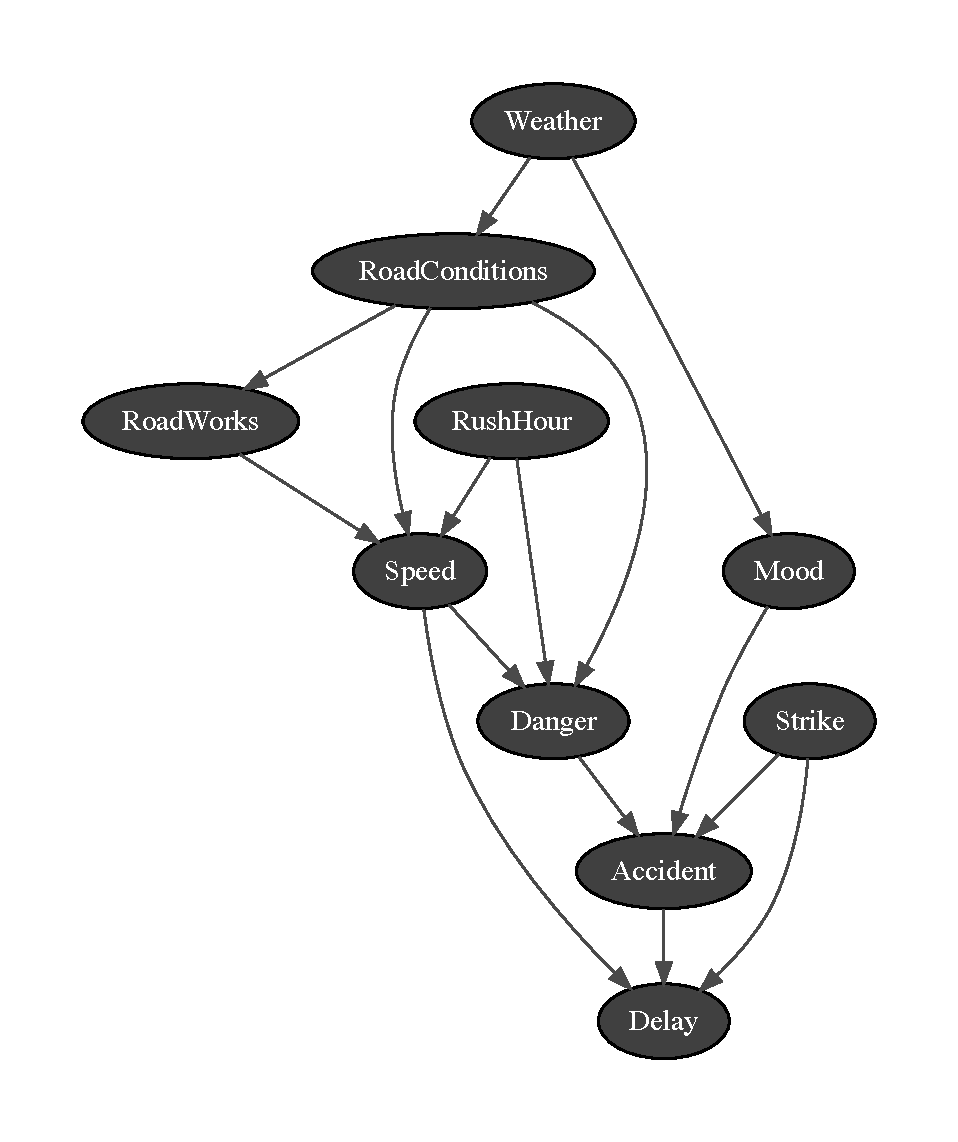
\includegraphics[width=\linewidth]{../code/network.pdf}	
	\caption{Bayesian Network}
	\label{fig:net}
\end{figure}

An arc can be inverted if and only if no v-structures, i.e. colliders in which the parents are not adjacent, are generated or destroyed in doing so.
 
In the model there are only two arrow that can be inverted, and these are the one that goes from the variable \texttt{Weather} to \texttt{Mood} and the one that goes from the variable \texttt{Weather} to \texttt{RoadConditions}.
In fact, even inverting the two arrows no v-structured are created, therefore the three graphs that are generated by the reversions of the two arcs are equivalent and not distinguishable by any statistical test.

Instead, the arc from \texttt{RoadWorks} to \texttt{RoadConditions} cannot be reverted since doing this a v-structure is created. Hence, the arc could only be turned on condition of turn also the one between 
\texttt{Weather} and \texttt{RoadConditions}.

\subsection*{D-Separation}
D-Separation tells when two variables are d-separated along a path (blocked), that means independent and when they are d-connected along a path (unblocked) or likely dependent.
They are actually independent if they are d-separated along all possible paths.
They are likely dependent if there is at least one unblocked path connecting them.

A path is blocked by a set of nodes if and only if the path contains a chain of nodes or a fork such that the middle node is in the set of nodes or if the path contains a collider such that the collision node and every descendant are not in the given set of nodes. 

\begin{itemize}
	\item X: \texttt{RushHour}, Y: \texttt{RoadConditions}:\\	
	Conditioning on one of the variables \texttt{Strike}, \texttt{RoadWorks} \texttt{Weather} or \texttt{Mood}, \texttt{RushHour} and \texttt{RoadConditions} are d-separated since the path from these two variables are all blocked.
	It is possible to write 
	\[ Y = \alpha + r_x X + r_a A + \epsilon \quad \text{with } r_a=0\]
	where A for example is \texttt{Strike}. 
	They are not actually independent since they are not d-separated along all the paths. For example, conditioning on one of the variables \texttt{Danger},\texttt{Speed}, \texttt{Accident} and \texttt{Delay}, the path from X to Y contains a collider in which the evidence is a collision node.
	In fact, all the variables d-connected are dependent in the real problem, for example \texttt{RushHour}, \texttt{RoadConditions} and \texttt{Danger}, while \texttt{RushHour}, \texttt{RoadConditions} and \texttt{Mood} are independent.
	
	\item X: \texttt{RushHour}, Y: \texttt{Strike}:\\
	Conditioning on one of the variables \texttt{Danger}, \texttt{RoadWorks}, \texttt{Weather}, \texttt{Speed} or \texttt{Mood}, \texttt{RushHour} and \texttt{Strike} are d-separated since the path from these two variables are all blocked.
	Instead, they are not d-separated along the paths that condition on variables \texttt{Accident} and \texttt{Delay} since in both the cases the paths contain a collider in which the given is the collision node. Hence, they are not independent.
	In the real problem, in fact, the d-connected variables are dependent, for example \texttt{RushHour}, \texttt{Strike} and \texttt{Danger}, while \texttt{RushHour}, \texttt{Strike} and \texttt{RoadWorks} are independent.
	
	\item X: \texttt{Speed}, Y: \texttt{Accident}:\\
	Are not d-separated given any of the variables of the domain.
	%FIXME
	"Danger", "Mood", "RoadConditions"
	
	\item X: \texttt{RoadConditions}, Y: \texttt{Strike}:\\
	In this case the same considerations made for the variables \texttt{RushHour} and \texttt{Strike} in example 2 apply.
	
	\item X: \texttt{Speed}, Y: \texttt{Mood}:\\
	Conditioning on one of the variables \texttt{RoadConditions} or \texttt{Weather}, \texttt{Speed} and \texttt{Mood} are d-separated since the path from these two variables are all blocked.
	Instead, they are not d-separated along the paths that condition on all the other variables, so they are not independent.
	The d-connected variables, for example \texttt{Speed}, \texttt{Mood} and \texttt{Danger}, are dependent in the real problem, while \texttt{Speed}, \texttt{Mood} and \texttt{RoadConditions} are not dependent.

\end{itemize}

\section{Conditional Probability Tables}

The Conditional Probability Tables (CPTs) of the variables of the model, that show all possible inputs and outcomes with their associated probabilities, are filled sometimes using information retrieved from online survey, other times are estimated based on common sense.
In case of the variable \texttt{Weather}, the prior probability is difficult to estimate because it is dependent on different factors, such as the location. For this reason I decided to use some information retrieved online\footlabel{note1}{\url{https://www.climatestotravel.com/climate/switzerland}} about the average precipitation in Lugano. Also the probabilities associated to the variable \texttt{Strike} are obtained from internet and referred to the number of strike of the public transport in Lugano.


\begin{figure}[H]
	\begin{center}	
	\begin{minipage}[c]{.3\textwidth}
		\centering
		
\includegraphics[width=.5\linewidth]{../code/strike.pdf}	
		\caption*{Strike CPT}
		\label{fig:strike}
	\end{minipage}
	~
	\begin{minipage}[c]{.3\textwidth}
		\centering
		
\includegraphics[width=.5\linewidth]{../code/weather.pdf}	
		\caption*{Weather CPT}
		\label{fig:weather}
	\end{minipage}
	~
	\begin{minipage}[c]{.3\textwidth}
		\centering
		
\includegraphics[width=.5\linewidth]{../code/rushhour.pdf}	
		\caption*{RushHour CPT}
		\label{fig:rushhour}
	\end{minipage}

	\begin{minipage}[c]{.31\textwidth}
		\centering
		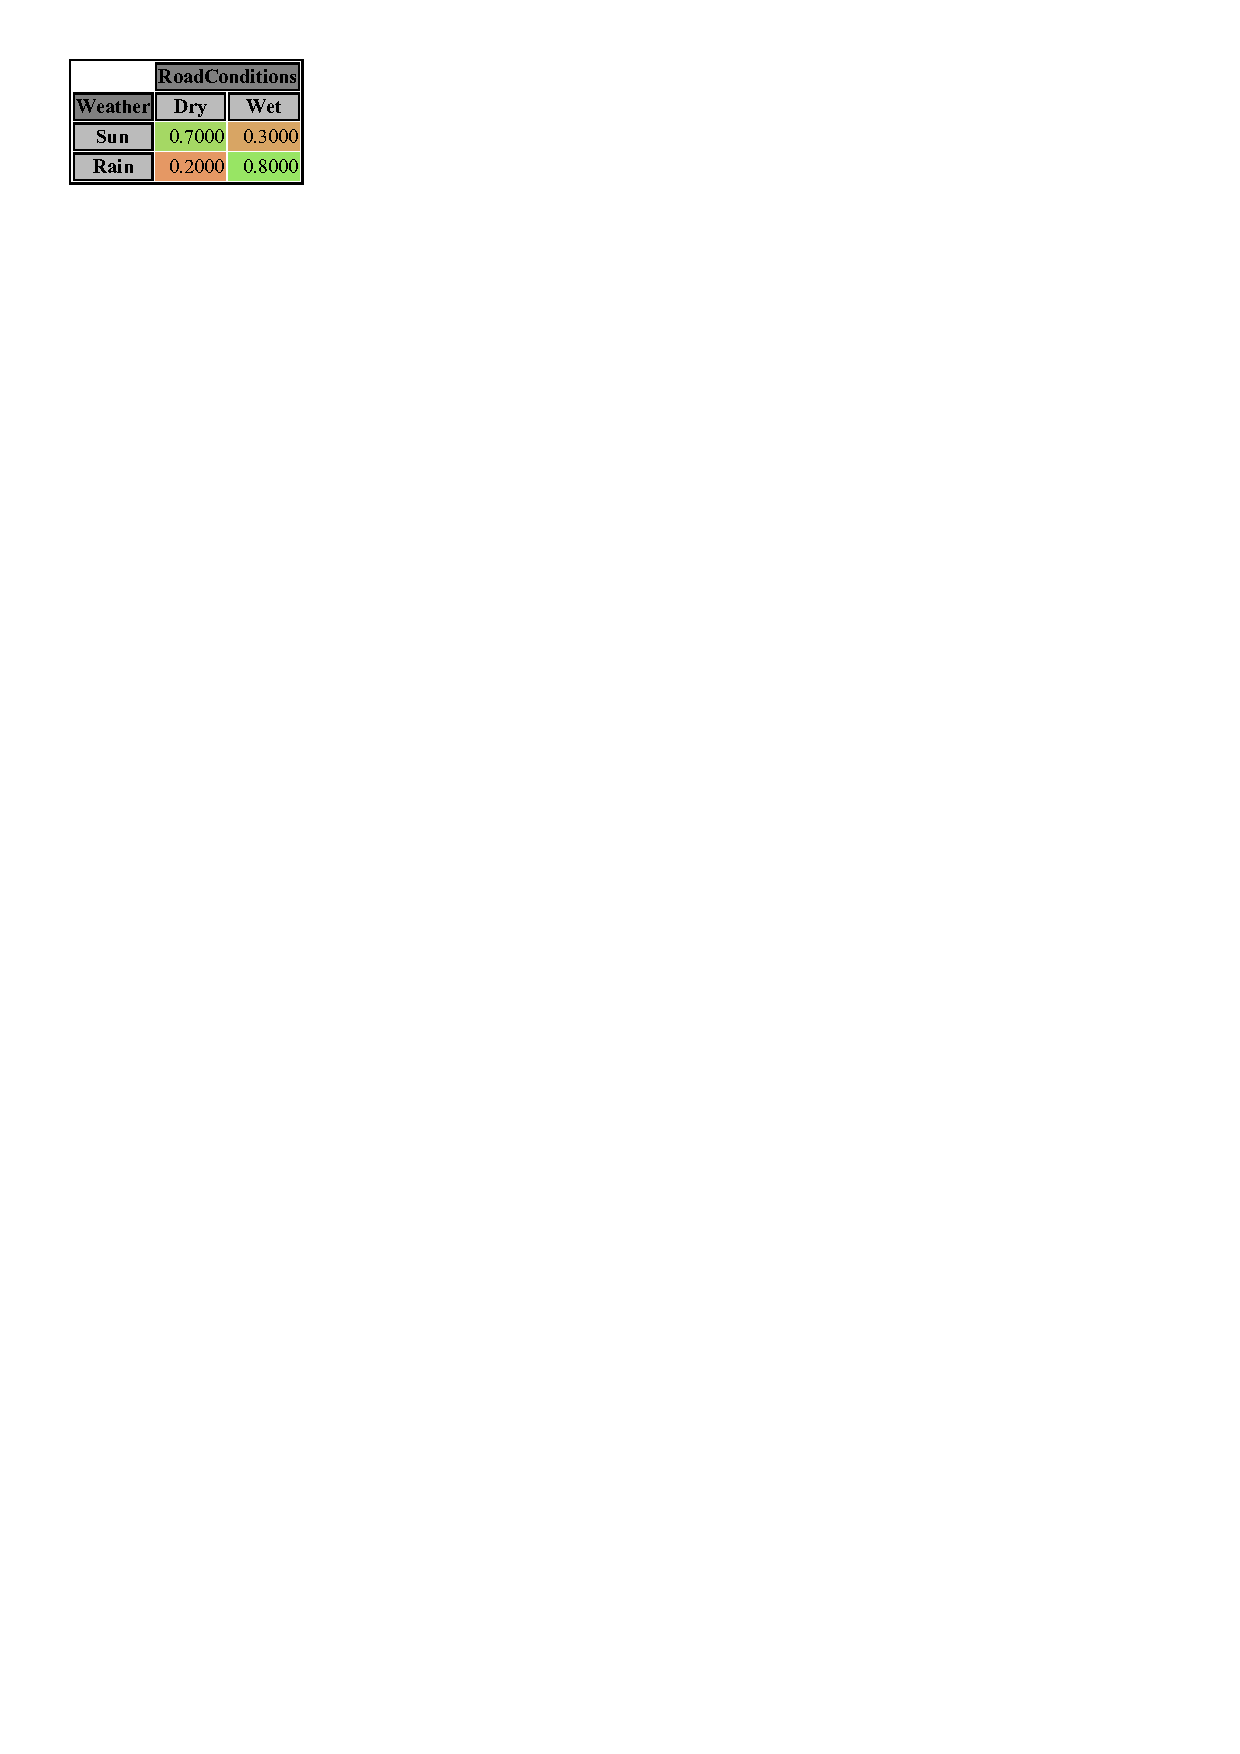
\includegraphics[width=.9\linewidth]{../code/roadconditions.pdf}	
		\caption*{RoadConditions CPT}
		\label{fig:roadconditions}
	\end{minipage}
	~
	\begin{minipage}[c]{.28\textwidth}
		\centering
		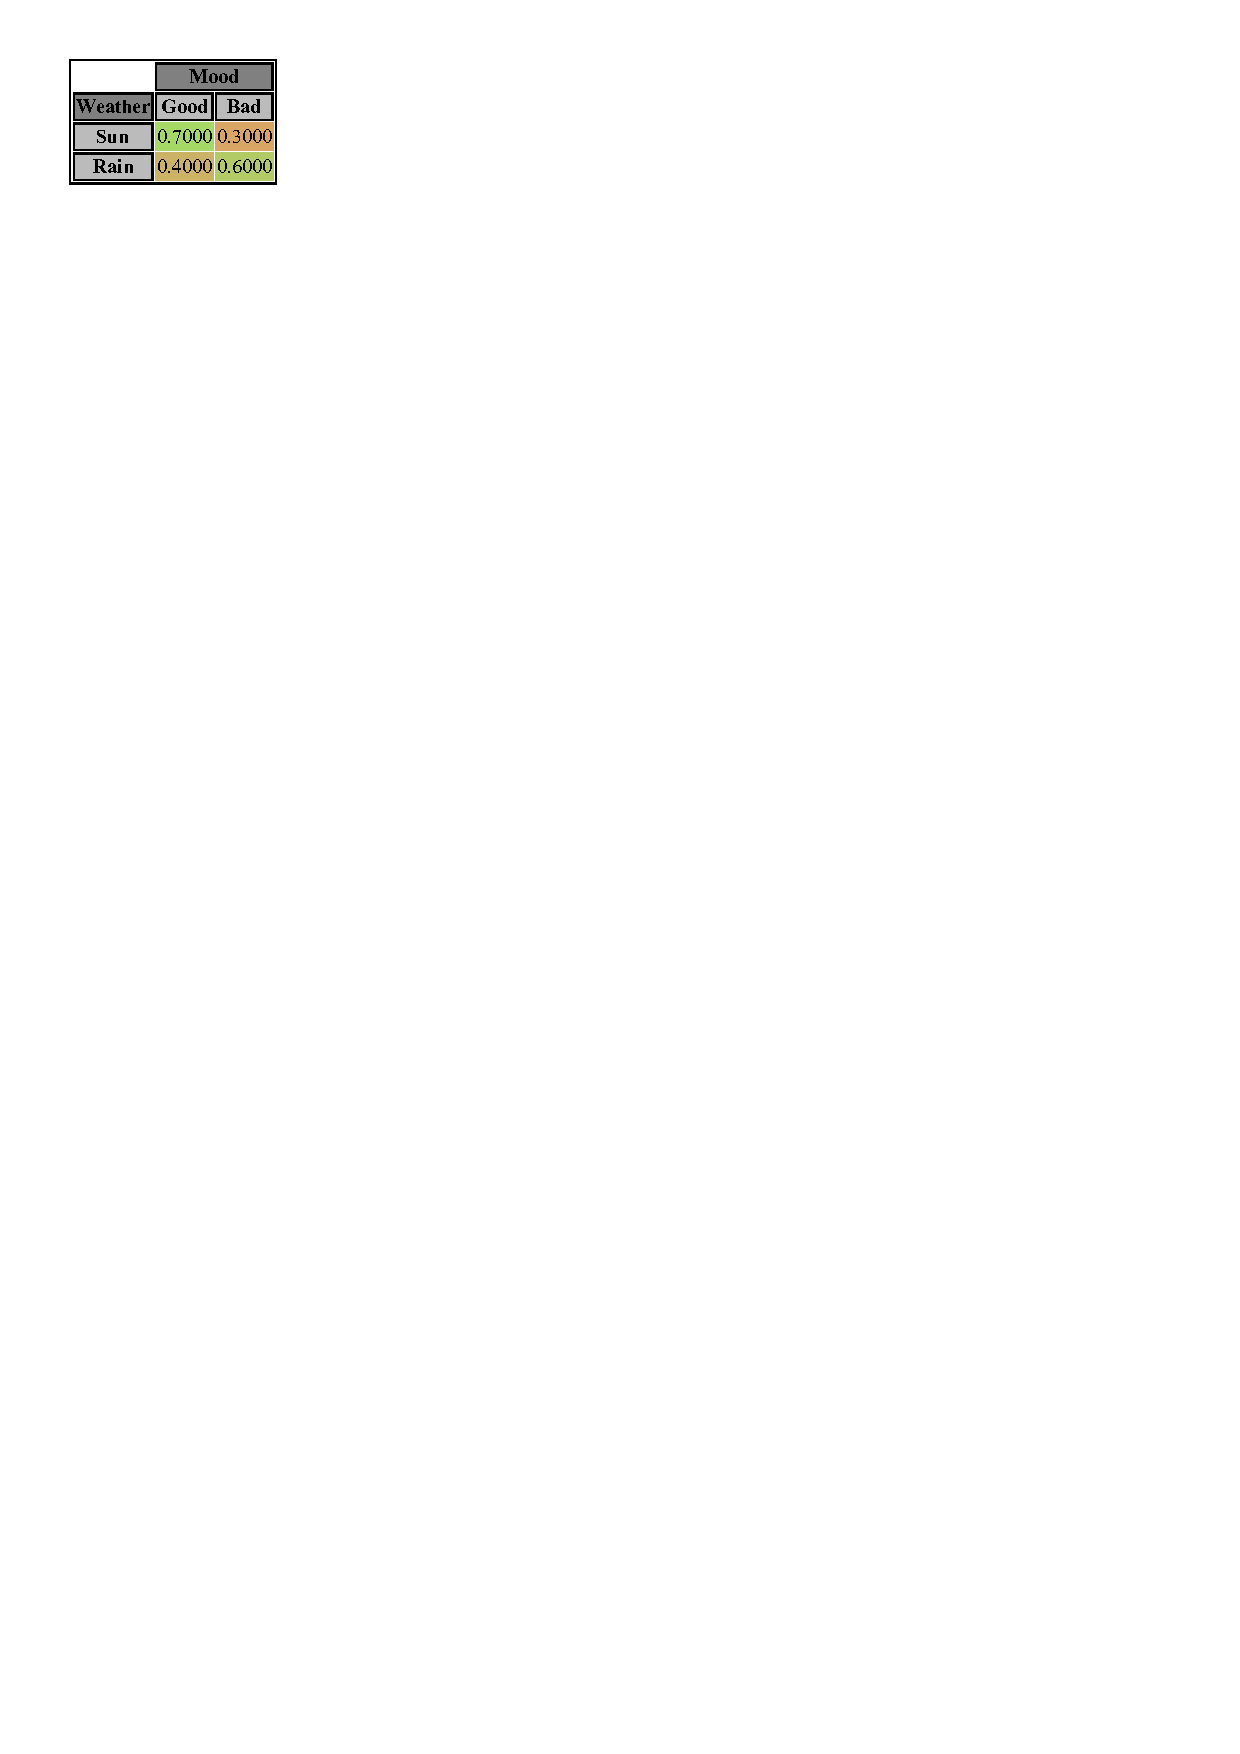
\includegraphics[width=.9\linewidth]{../code/mood.pdf}	
		\caption*{Mood CPT}
		\label{fig:Mood}
	\end{minipage}
	~
	\begin{minipage}[c]{.35\textwidth}
		\centering
		
		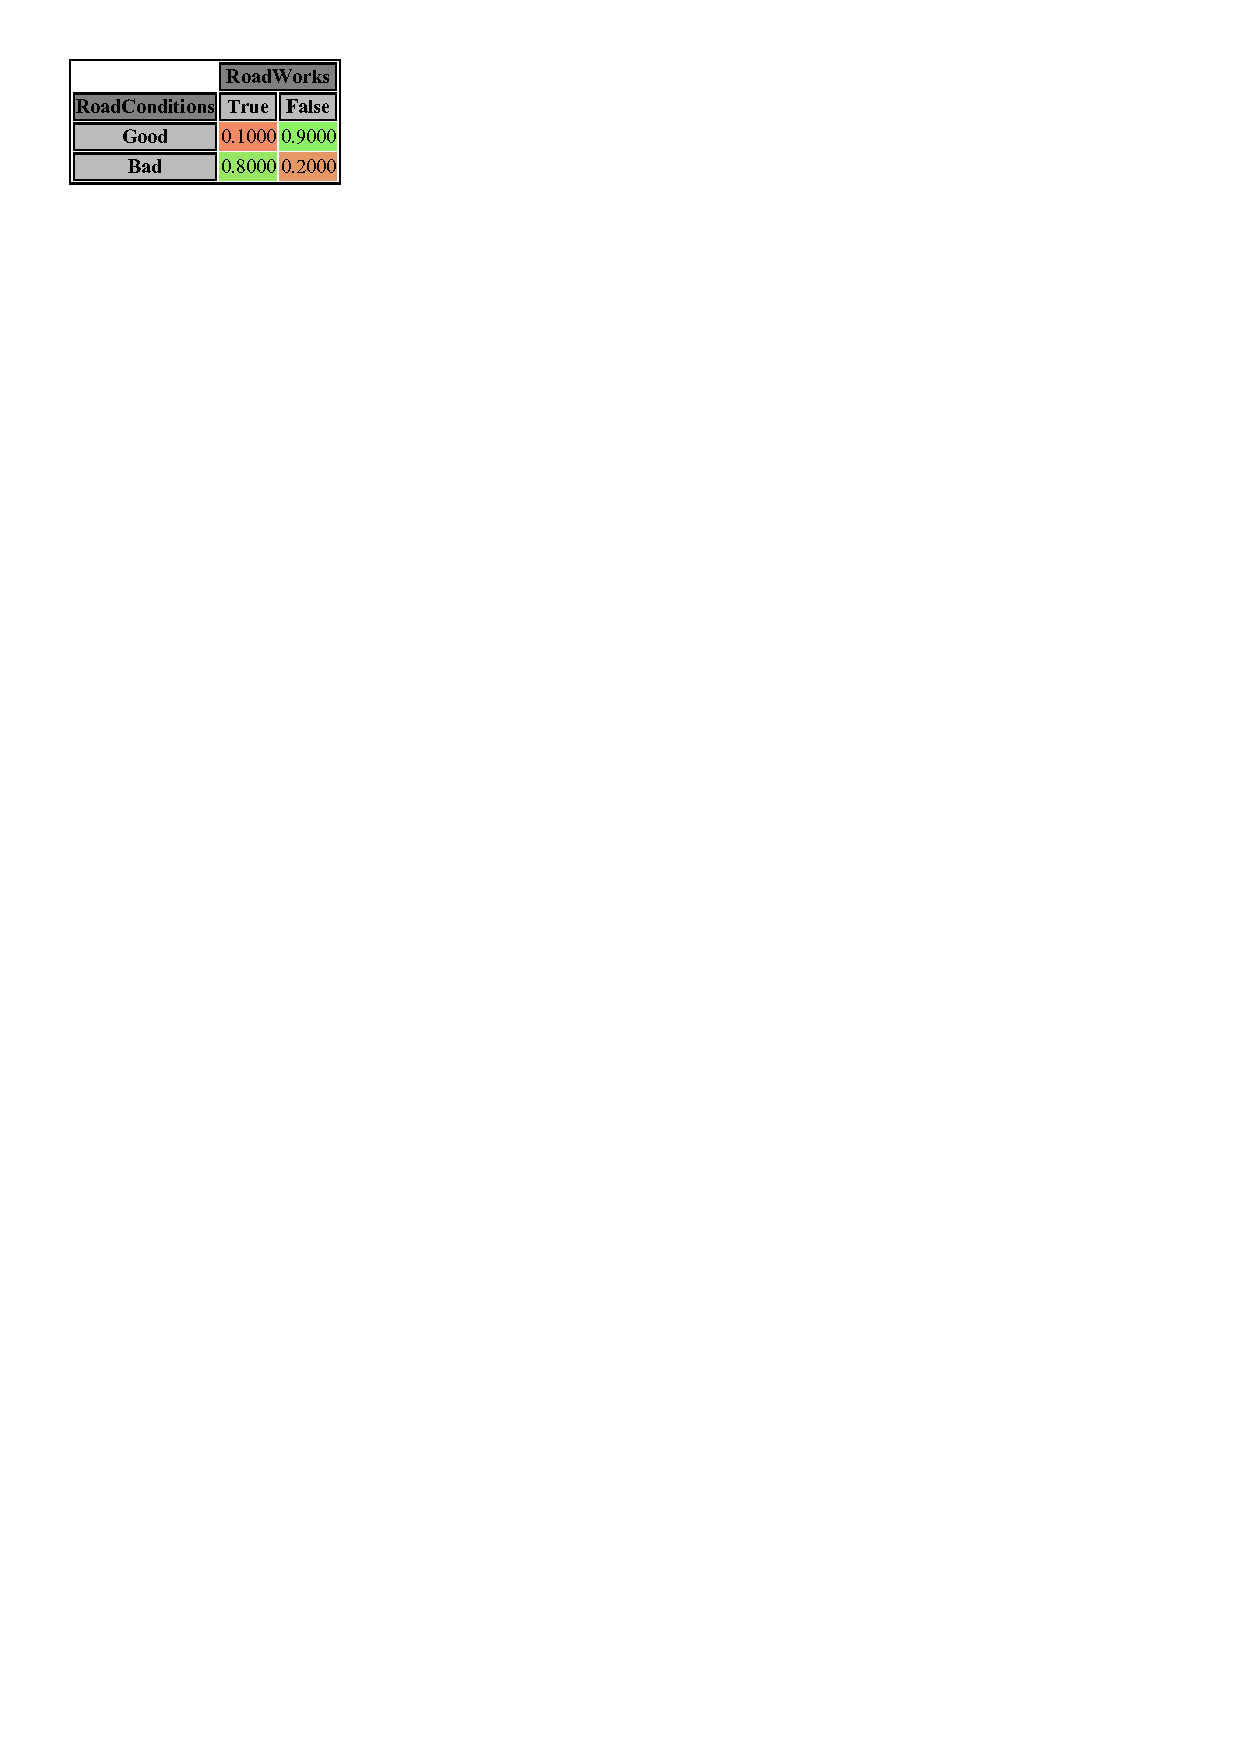
\includegraphics[width=.9\linewidth]{../code/roadworks.pdf}	
		\caption*{RoadWorks CPT}
		\label{fig:roadworks}
	\end{minipage}

	\begin{minipage}[c]{.5\textwidth}
		\centering
		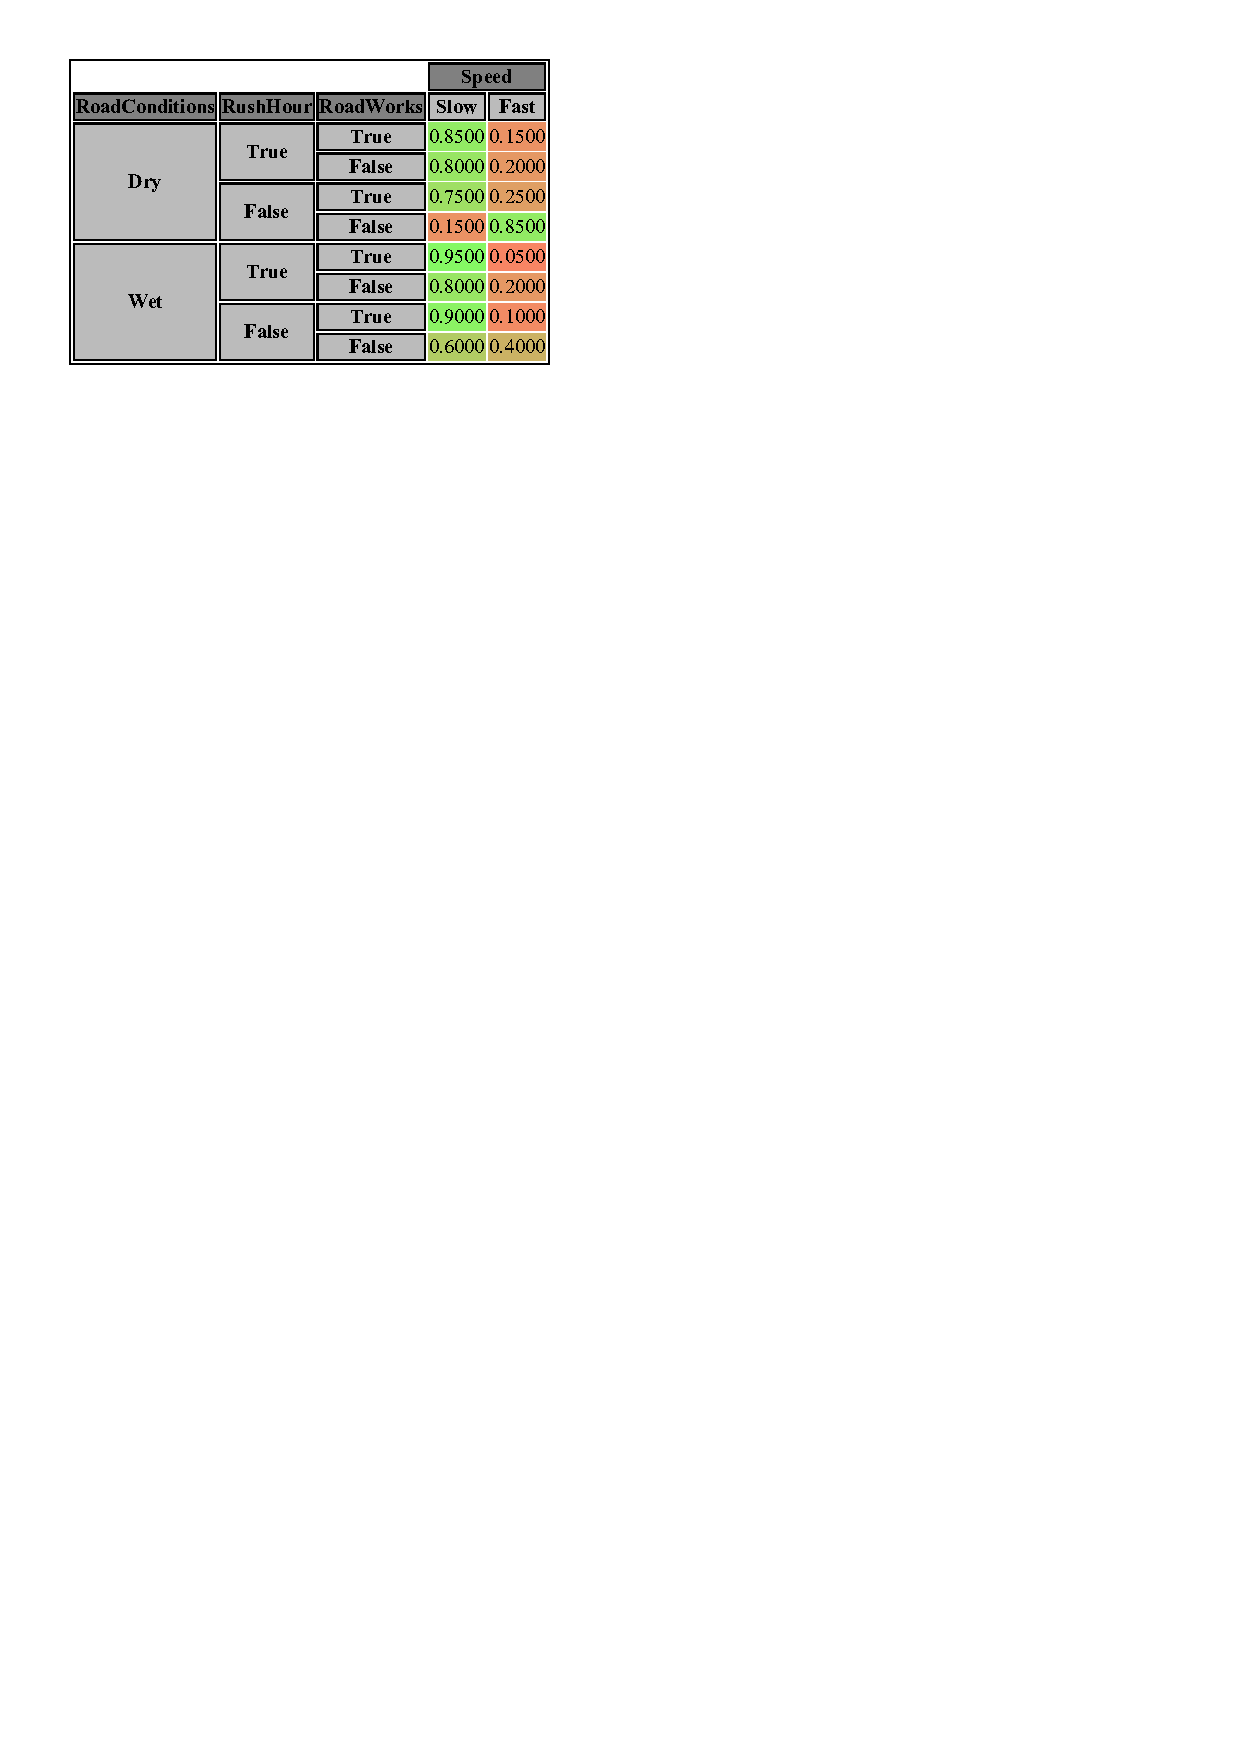
\includegraphics[width=\linewidth]{../code/speed.pdf}	
		\caption*{Speed CPT}
		\label{fig:speed}
	\end{minipage}
	~
	\begin{minipage}[c]{.45\textwidth}
		\centering
		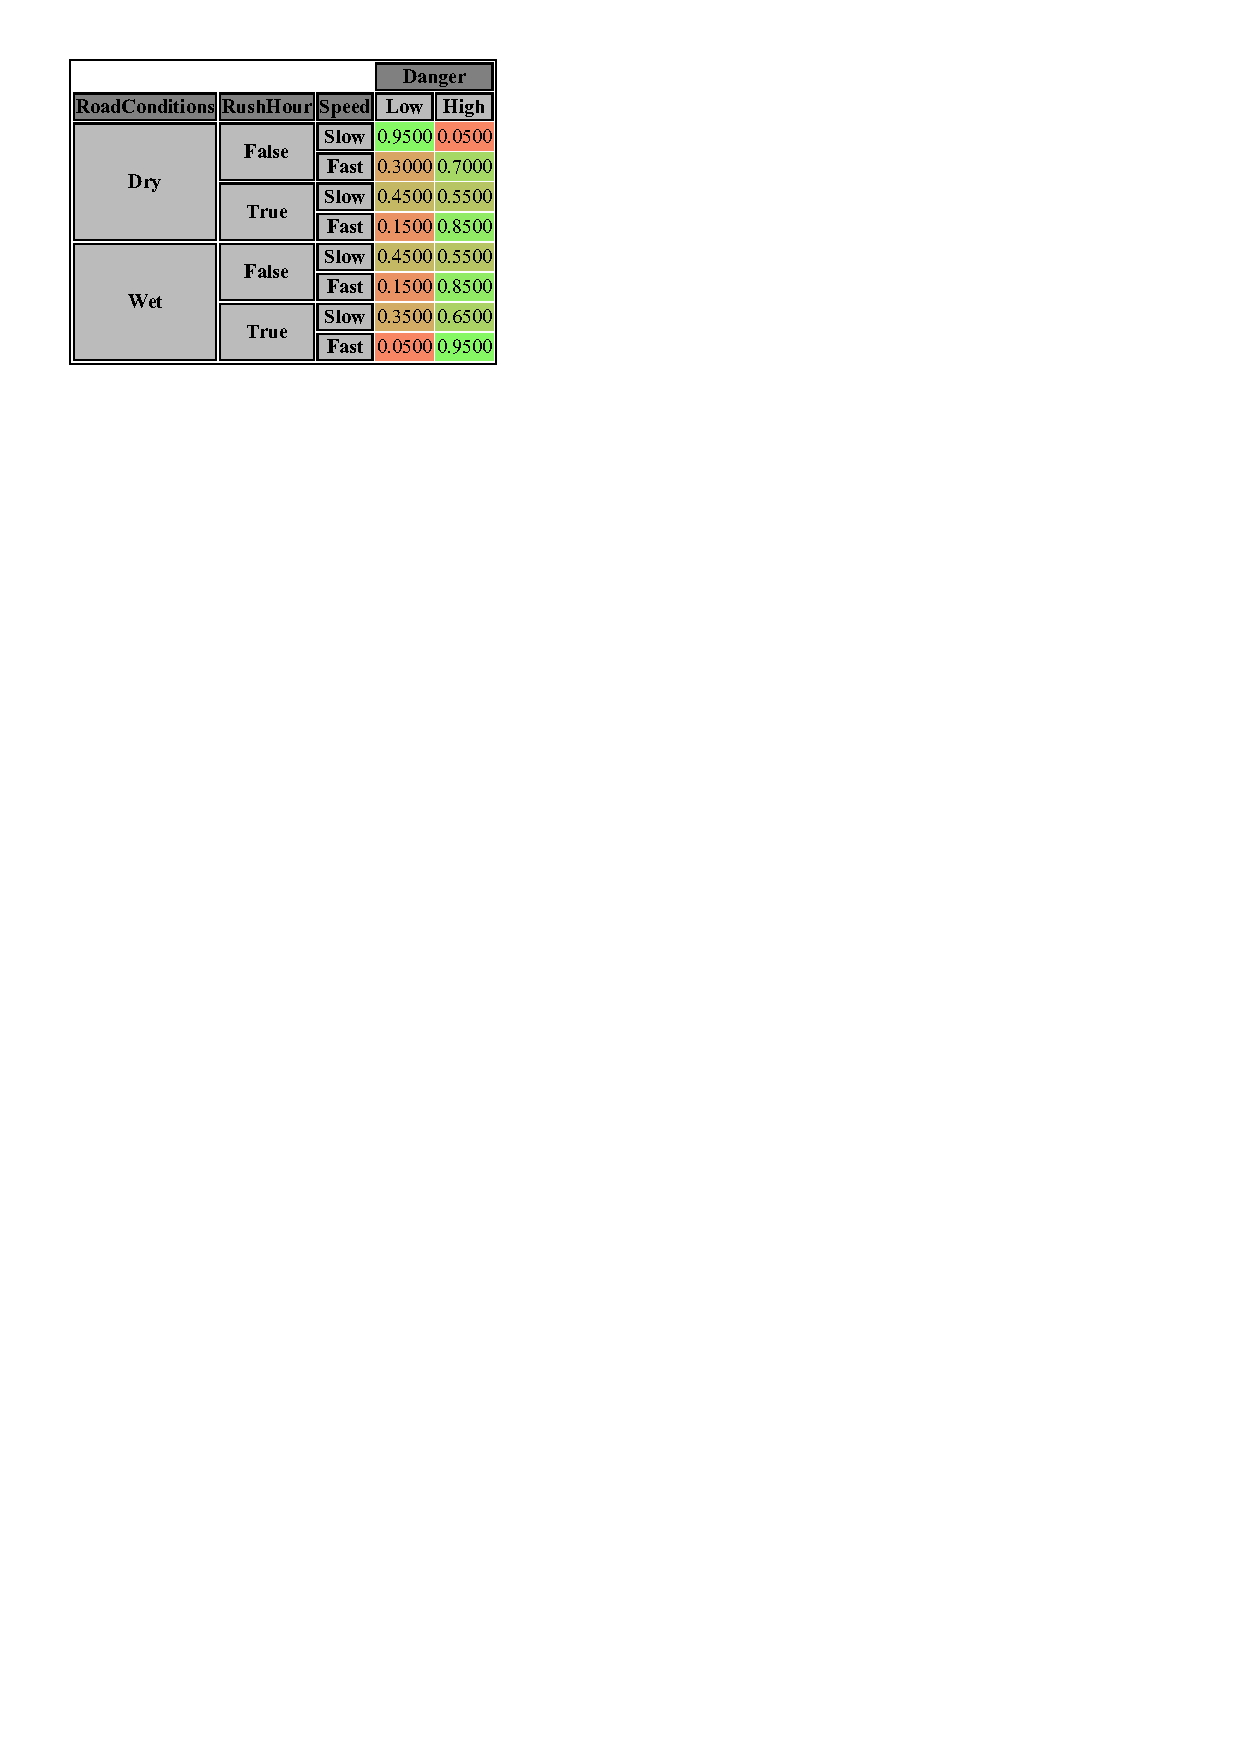
\includegraphics[width=\linewidth]{../code/danger.pdf}	
		\caption*{Danger CPT}
		\label{fig:danger}
	\end{minipage}
	\end{center}
	\end{figure}
	
	\begin{figure}[H]
	\begin{center}
	\centering
	\begin{minipage}[c]{.45\textwidth}
		\centering
		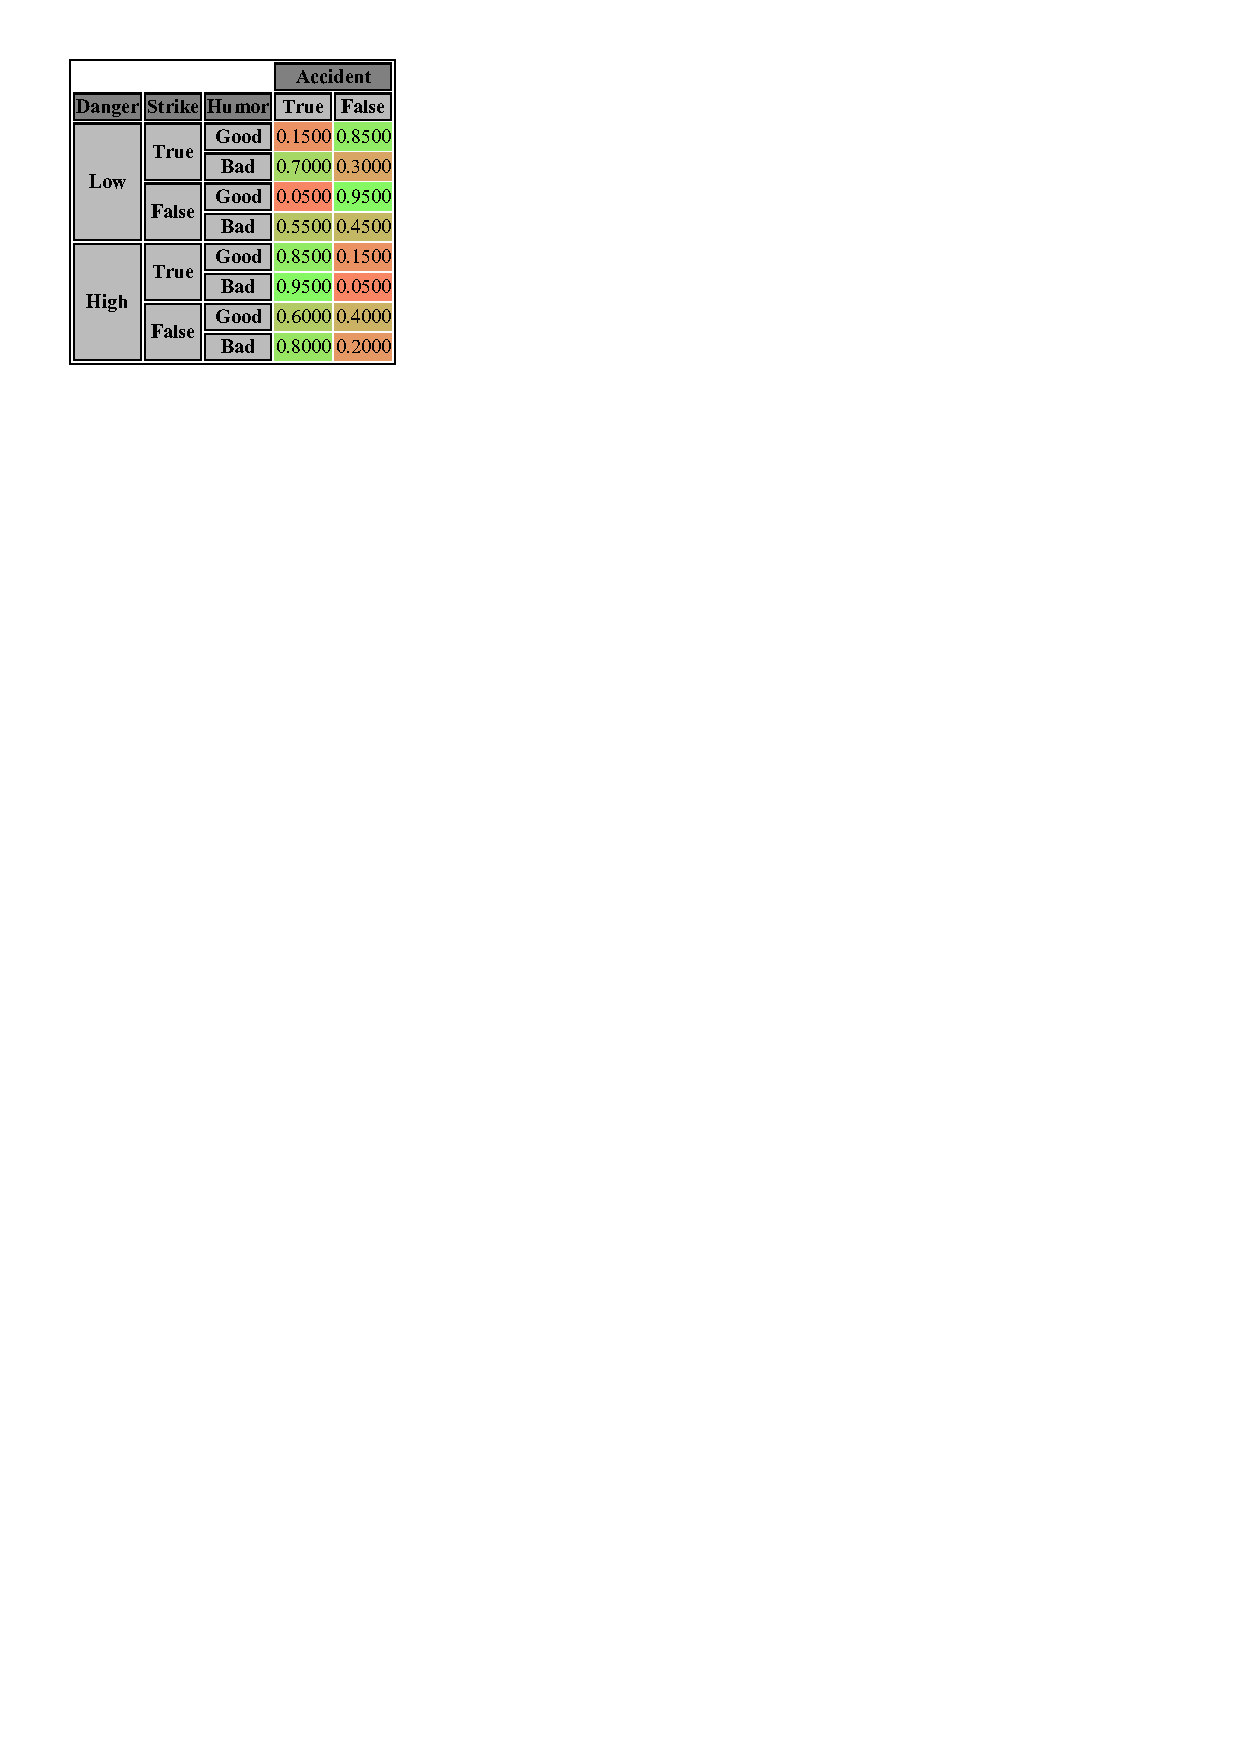
\includegraphics[width=.9\linewidth]{../code/accident.pdf}	
		\caption*{Accident CPT}
		\label{fig:accident}
	\end{minipage}
	~
	\begin{minipage}[c]{.45\textwidth}
		\centering
		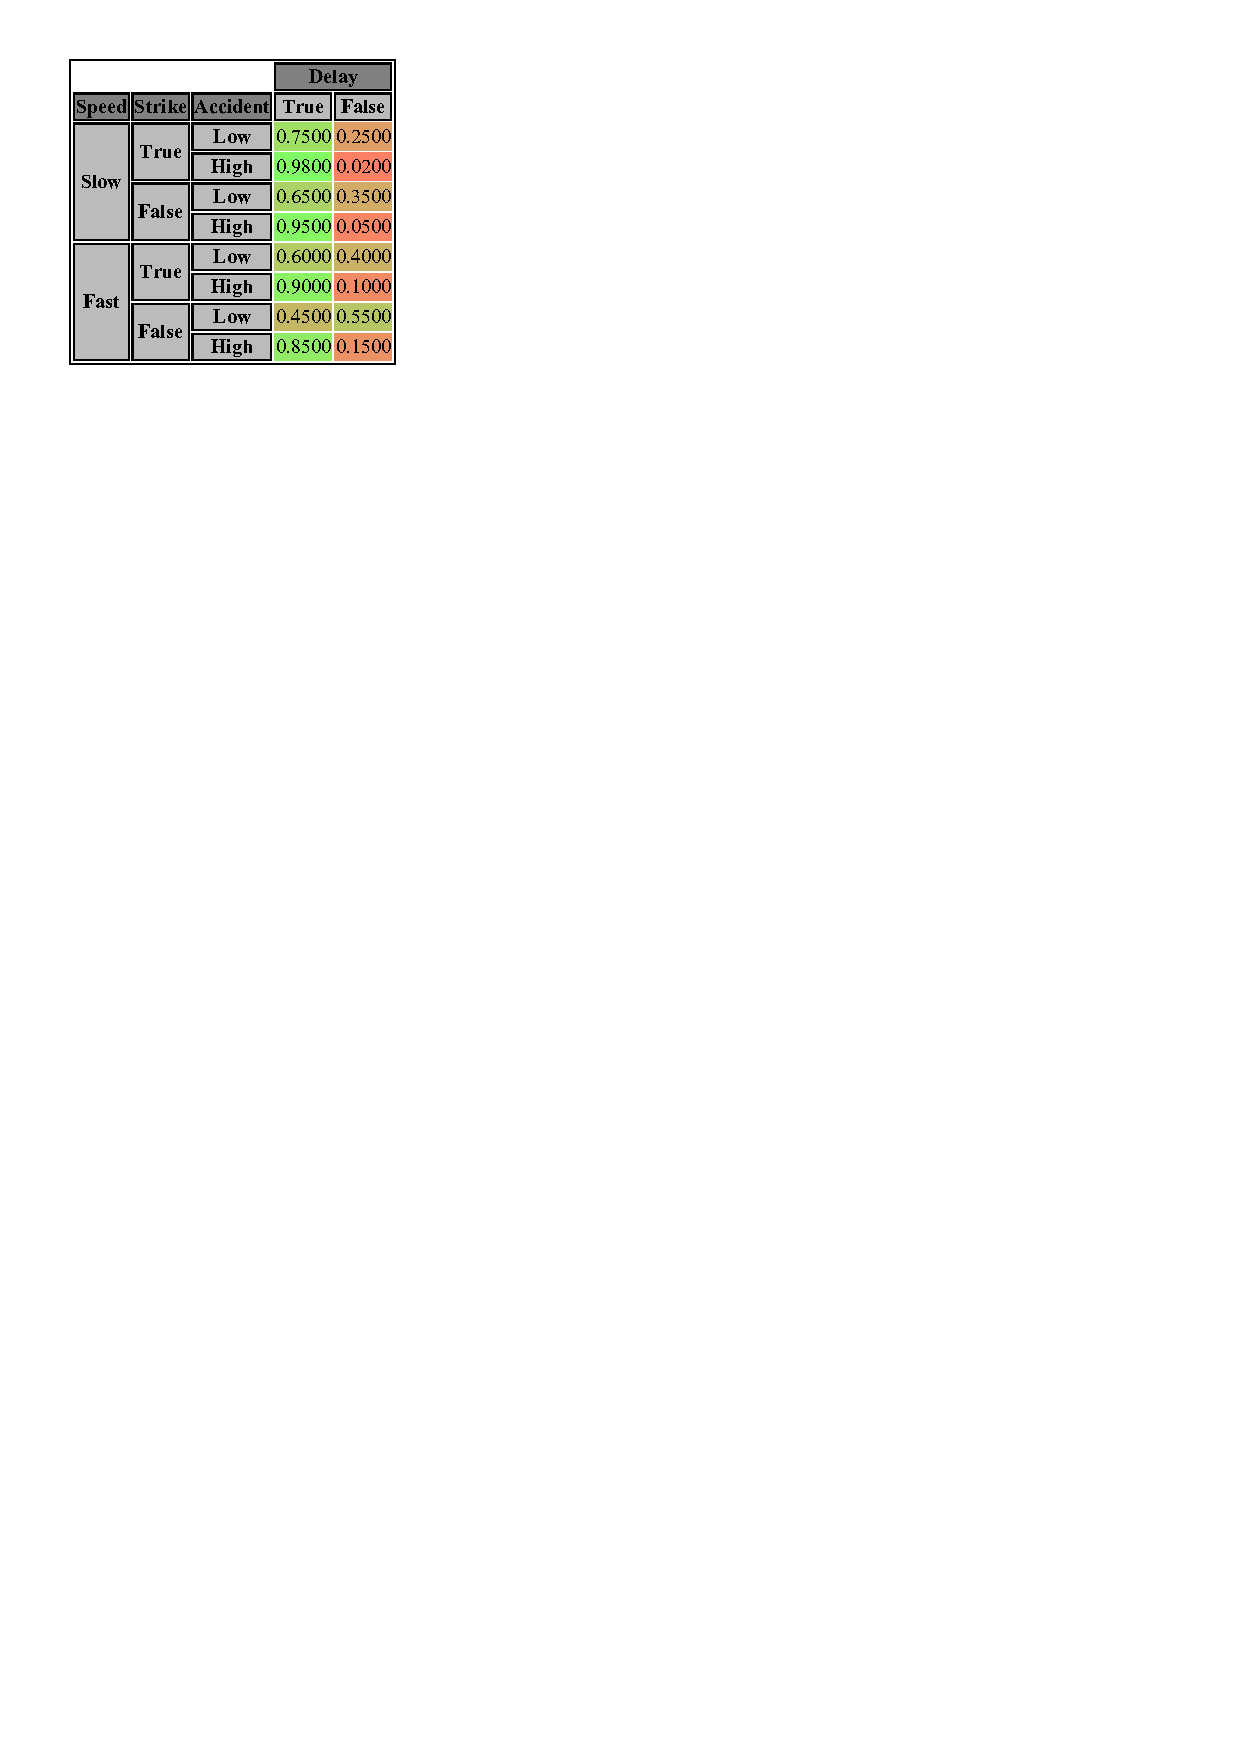
\includegraphics[width=.9\linewidth]{../code/delay.pdf}	
		\caption*{Delay CPT}
		\label{fig:delay}
	\end{minipage}

\end{center}
\end{figure}

\section{Causal Inference}

\subsection*{Causal Effect}
Given the graph, and a pair of variables \texttt{X}: \texttt{Speed} and \texttt{Y}: \texttt{Accident}. In this case, \texttt{A}: \texttt{RoadConditions} and \texttt{B}: \texttt{RushHour} are the backdoor variables. Then the causal effect of \texttt{X} on \texttt{Y} is given by the following formula:
\begin{equation}
	\text{P}(Y = y \mid {do}(X = x)) = \sum_{A}^{}\sum_{B}^{}	\text{P}(Y = y \mid X = x, A = a, B = b)\text{P}(A = a, B = b)
\end{equation}
where $a$, $b$, $y$ and $x$ range over all the combinations of values that the associated variable can take.\\

\noindent Calculating the cases in which $\mathtt{Y}: \{ y_0=\mathtt{false}, y_1=\mathtt{true}\}$ given $\mathtt{X}: \{ x_0=\mathtt{slow}, x_1=\mathtt{fast}\}$ :
\begin{equation*}
\begin{aligned}
\text{P}(y_0 \mid {do}(x_0)) = \sum_{A}^{}\sum_{B}^{}	\text{P}(y_0 \mid x_0, A = a, B = b)\text{P}(A = a, B = b)  = 0.6062	
\\
\text{P}(y_1 \mid {do}(x_0)) = \sum_{A}^{}\sum_{B}^{}	\text{P}(y_1 \mid x_0, A = a, B = b)\text{P}(A = a, B = b) = 0.3938
\\
\text{P}(y_0 \mid {do}(x_1)) = \sum_{A}^{}\sum_{B}^{}	\text{P}(y_0 \mid x_1, A = a, B = b)\text{P}(A = a, B = b) =  0.4053	
\\
\text{P}(y_1 \mid {do}(x_1)) = \sum_{A}^{}\sum_{B}^{}	\text{P}(y_1 \mid x_1, A = a, B = b)\text{P}(A = a, B = b) =  0.5947
\end{aligned}
\end{equation*}

\subsection*{Confounders}
Given the variables \texttt{X}: \texttt{Speed} and \texttt{Y}: \texttt{Accident}, they do not have any confounder. In fact, the possible confounders can be identified searching for the parents of \texttt{X}, that are \texttt{RoadWorks}, \texttt{RoadConditions} and \texttt{RushHour}, but none of this variables is a parent of \texttt{Y}, so they do not have any confounder.

\subsection*{Randomised Controlled Study}
%FIXME
With this specific problem is not possible to perform randomised controlled study on every variable. For example, we cannot influence the weather, so randomise variables affecting \texttt{RoadConditions} or \texttt{Mood} is impossible.

By the way, if we are interested in performing a randomised controlled study to disentangle the causal effect between \texttt{X}: \texttt{Speed} and \texttt{Y}: \texttt{Accident} from their correlation it is necessary to fix or vary randomly the variable \texttt{X}. In this case is possible to fix the driving velocity by introducing for example a speed limit.
%then what happen?

\subsection*{Average Causal Effect}
The Average Causal Effect (ACE) of X on Y is computed for both the possible values of the variable \texttt{Accident}, that are $\mathtt{Y}: \{ y_0=\mathtt{false}, y_1=\mathtt{true}\}$ 
\begin{equation}
\begin{aligned}
\text{ACE}&=\text{P}(y_0 \mid {do}(x_0)) -\text{P}(y_0 \mid {do}(x_1)) \approx -0.189
\\
\text{ACE}&=\text{P}(y_1 \mid {do}(x_0)) -\text{P}(y_1 \mid {do}(x_1)) \approx 0.189
\end{aligned}
\end{equation}


\subsection*{C-Specific Effect}
%Using the same \texttt{X} and \texttt{Y} as before, and chosen \texttt{C}: \texttt{RushHour}.
%The C-Specific Effect if given by:
%\begin{equation}
%	P(Y=y|do(X=x), C=c)= \sum_{z} P(Y=y|X=x, C=c, Z=z) P(Z=z|C=c)
%\end{equation}
%The set Z identified such that $C \cup Z$ satisfy the backdoor criterion is composed by the variables \texttt{Danger}, \texttt{Mood}, \texttt{RoadConditions}, \texttt{Strike}, \texttt{Weather}.\newline
%Defined $\mathtt{X}: \{ x_0=\mathtt{slow}, x_1=\mathtt{fast}\}$, $\mathtt{Y}: \{ y_0=\mathtt{false}, y_1=\mathtt{true}\}$ and $\mathtt{C}: \{ c_0=\mathtt{false}, c_1=\mathtt{true}\}$ it is possible to compute the C-Specific Effect for all the possible realisation of the variables as follows: 
%
%\begin{equation*}
%P(y_0|do(x_0), c_0)= \sum_{z} P(y_0|x_0, c_0, z) P(z|c_0)=0.4914
%\end{equation*}
%
%\begin{equation*}
%P(y_1|do(x_0), c_0)= \sum_{z} P(y_1|x_0, c_0, z) P(z|c_0)=0.5086
%\end{equation*}
%
%\begin{equation*}
%P(y_0|do(x_1), c_0)= \sum_{z} P(y_0|x_1, c_0, z) P(z|c_0)=0.3604
%\end{equation*}
%
%\begin{equation*}
%P(y_1|do(x_1), c_0)= \sum_{z} P(y_1|x_1, c_0, z) P(z|c_0)=0.6396
%\end{equation*}
%
%\begin{equation*}
%P(y_0|do(x_0), c_1)= \sum_{z} P(y_0|x_0, c_1, z) P(z|c_1)=0.6350
%\end{equation*}
%
%\begin{equation*}
%P(y_1|do(x_0), c_1)= \sum_{z} P(y_1|x_0, c_1, z) P(z|c_1)=0.3650
%\end{equation*}
%
%\begin{equation*}
%P(y_0|do(x_1), c_1)= \sum_{z} P(y_0|x_1, c_1, z) P(z|c_1)=0.4165
%\end{equation*}
%
%\begin{equation*}
%P(y_1|do(x_1), c_1)= \sum_{z} P(y_1|x_1, c_1, z) P(z|c_1)=0.5835
%\end{equation*}
%
%The minimal set of variables that must be measured in order to estimate the c-specific effect of X on Y includes \texttt{Speed}, \texttt{Accident}, \texttt{RushHour} and \texttt{RoadConditions}.
Given a new pair of variable such that \texttt{X}: \texttt{Danger} and \texttt{Y}: \texttt{Delay}, and chosen \texttt{C}: \texttt{RoadConditions}, the C-Specific Effect is given by:
\begin{equation}
P(Y=y|do(X=x), C=c)= \sum_{z} P(Y=y|X=x, C=c, Z=z) P(Z=z|C=c)
\end{equation}
The set Z identified, such that $C \cup Z$ satisfy the backdoor criterion, includes the variable \texttt{Speed}.
Defined $\mathtt{X}: \{ x_0=\mathtt{low}, x_1=\mathtt{high}\}$, $\mathtt{Y}: \{ y_0=\mathtt{false}, y_1=\mathtt{true}\}$ and $\mathtt{C}: \{ c_0=\mathtt{dry}, c_1=\mathtt{wet}\}$ it is possible to compute the C-Specific Effect for all the possible realisation of the variables as follows: 

\begin{equation*}
P(y_0|do(x_0), c_0)= \sum_{z} P(y_0|x_0, c_0, z) P(z|c_0)=0.6150
\end{equation*}

\begin{equation*}
P(y_1|do(x_0), c_0)= \sum_{z} P(y_1|x_0, c_0, z) P(z|c_0)=0.3850
\end{equation*}

\begin{equation*}
P(y_0|do(x_1), c_0)= \sum_{z} P(y_0|x_1, c_0, z) P(z|c_0)=0.2866
\end{equation*}

\begin{equation*}
P(y_1|do(x_1), c_0)= \sum_{z} P(y_1|x_1, c_0, z) P(z|c_0)=0.7134
\end{equation*}

\begin{equation*}
P(y_0|do(x_0), c_1)= \sum_{z} P(y_0|x_0, c_1, z) P(z|c_1)=0.5633
\end{equation*}

\begin{equation*}
P(y_1|do(x_0), c_1)= \sum_{z} P(y_1|x_0, c_1, z) P(z|c_1)=0.4367
\end{equation*}

\begin{equation*}
P(y_0|do(x_1), c_1)= \sum_{z} P(y_0|x_1, c_1, z) P(z|c_1)=0.2662
\end{equation*}

\begin{equation*}
P(y_1|do(x_1), c_1)= \sum_{z} P(y_1|x_1, c_1, z) P(z|c_1)=0.7338
\end{equation*}

\begin{figure}[H]
	\centering
	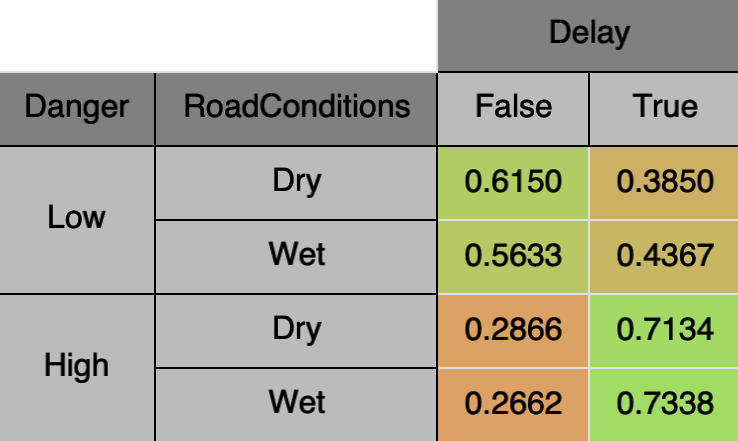
\includegraphics[width=.5\linewidth]{../code/c-specific-effect.png}	
	\caption*{CPT C-Specific Effect}
	\label{fig:c-specific-effect}
\end{figure}
	%FIXME
The minimal set of variables that must be measured in order to estimate the c-specific effect of X on Y includes \texttt{Danger}, \texttt{Delay}, \texttt{Speed} and \texttt{RoadConditions}.
\subsection*{Conditional Intervention}
Given \texttt{X}: \texttt{Danger} and \texttt{Y}: \texttt{Delay}, and chosen \texttt{C}: \texttt{RoadConditions}, the Conditional Intervention in which we are interested is:

$$P(Y=y|do(X=g(C)))$$

where $$ g(C) := \left\{\begin{array}{lr}
low, & \text{if } C=dry\\
high, & \text{if } C=wet
\end{array}\right\}$$
Then the conditional intervention is computed using 
\begin{equation}
	P(Y=y|do(X=g(C))) = \sum_c P(Y=y|do(X=g(C)), C=c)P(C=c)
\end{equation}
$$$$

\subsection*{Mediation and Controlled Direct Effect}
Given a new pair of variable such that \texttt{X}: \texttt{RushHour} and \texttt{Y}: \texttt{Danger}, the variable \texttt{M}: \texttt{Speed} is a mediation variable between \texttt{X} and \texttt{Y}.
The Controlled Direct Effect is computed with the following formula:
\begin{equation}
	\text{CDE} = P(Y = y|\mathrm{do}(X = x),\mathrm{do}(M = m)) - P(Y = y|\mathrm{do}(X = x'),\mathrm{do}(M = m))
\end{equation}
Since there are not any spurious path between X and Y, the formula can be rewritten as follows:
\begin{equation*}
\text{CDE} = P(y| x,\mathrm{do}( m)) - P(y|x',\mathrm{do}(m))
\end{equation*}
Then, applying the backdoor criterion it is possible to bock the spurious path between M and Y, in particular using \texttt{Z}: \texttt{RoadConditions} as backdoor variable. We should consider the variable \texttt{W}: \texttt{Weather} since is parent of Z.
Finally we obtain
\begin{equation*}
\text{CDE} = \bigg[\sum_{z,w}P(y| x,m, z)P(z|w)P(w)\bigg] - \bigg[\sum_{z,w}P(y| x',m, z)P(z|w)P(w)\bigg]
\end{equation*}

Defined $\mathtt{X}: \{ x_0=\mathtt{true}, x_1=\mathtt{false}\}$, $\mathtt{Y}: \{ y_0=\mathtt{low}, y_1=\mathtt{high}\}$, $\mathtt{M}: \{ m_0=\mathtt{slow}, m_1=\mathtt{fast}\}$ the CME are: 

\begin{equation*}
\text{CDE} = P(y_0|\mathrm{do}(x_0),\mathrm{do}(m_0)) - P(y_0|\mathrm{do}(x_1),\mathrm{do}(m_0)) = 0.1050 - 0.2330 = -0.128
\end{equation*}
\begin{equation*}
\text{CDE} = P(y_1|\mathrm{do}(x_0),\mathrm{do}(m_0)) - P(y_1|\mathrm{do}(x_1),\mathrm{do}(m_0))=0.8950 - 0.7675 = 0.128
\end{equation*}
\begin{equation*}
\text{CDE} = P(y_0|\mathrm{do}(x_0),\mathrm{do}(m_1)) - P(y_0|\mathrm{do}(x_1),\mathrm{do}(m_1))=0.405 - 0.725 = -0.31999999999999995
\end{equation*}
\begin{equation*}
\text{CDE} = P(y_1|\mathrm{do}(x_0),\mathrm{do}(m_1)) - P(y_1|\mathrm{do}(x_1),\mathrm{do}(m_1))=0.595 - 0.275 = 0.31999999999999995
\end{equation*}

 CDE of Y changing the value of X.

\section{Simulation}
Suppose that you can’t measure some parents of variable X chosen in every point of “Causal Inference”.
Repeat the “Causal Inference” part of the exercise considering this new situation.

\section{Comment on the Results}
What kind of experience have you got with this model? E.g., is the causal model responding in a sensible way to your queries? What should be changed/modified to make it more realistic?


\end{document}
